\section{Related Work}

\begin{frame}{Agricultural Remote Sensing: Sensors \& Spectral Behavior}
    \renewcommand{\currprop}{0.4\textheight}
    \begin{itemize}
    \item Remote Sensing heavily relies on capturing Electromagnetic Radiation (EMR).
    \pause
    \item Researchers use mathematical combinations of spectral bands to highlight vegetation health and age (e.g., NDVI, EVI2).
    \pause
    \item We can distinguish crop species because each plant has a unique spectral response curve 
    \end{itemize}

    \pause
    \begin{figure}
        \centering
        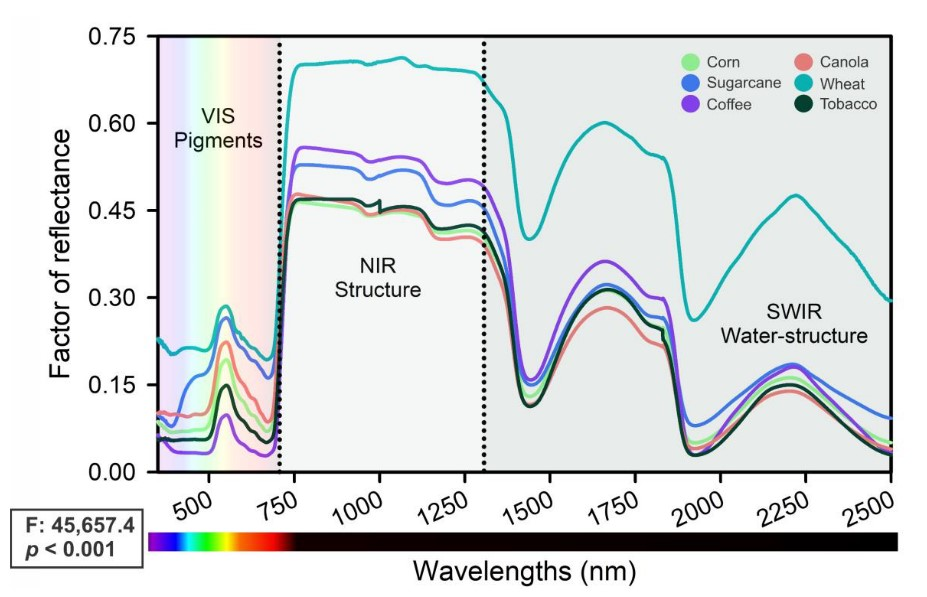
\includegraphics[height=\currprop]{figures/3_theoretical_background/veg_reflectance.jpg}
    \end{figure}
\end{frame}

\begin{frame}{Agricultural Remote Sensing: SITS \& Phenology}
    \renewcommand{\currprop}{0.5\textheight}
    \begin{block}{Satellite Image Time Series (SITS)}
        A single image is rarely enough for agriculture. SITS captures the temporal evolution of an agricultural parcel, revealing the crop's \textit{phenological cycle} (planting, growth peak, harvest).
    \end{block}
    \pause
        \begin{figure}
        \centering
        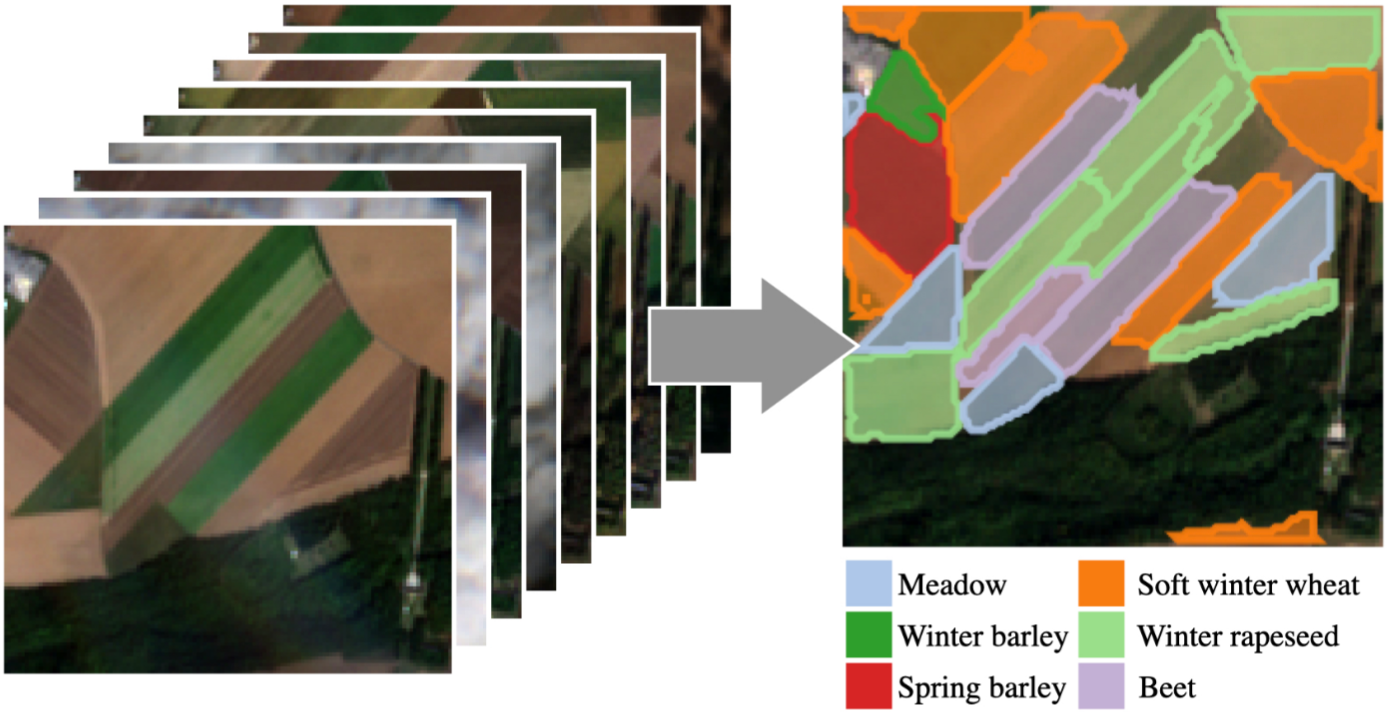
\includegraphics[height=\currprop]{figures/1_introduction/pastis-sits.png}
    \end{figure}
\end{frame}

\begin{frame}{Machine Learning: From Shallow to Deep Learning}
    \begin{block}{Shallow Learning (SL)}
        Traditional models like Random Forest (RF) and Support Vector Machines (SVM) require \textbf{Feature Engineering} (e.g., extracting monthly averages or hand-crafted indices) to process unstructured SITS data.
    \end{block}
    \pause
    \begin{block}{Deep Learning (DL)}
        Deep architectures (CNNs, LSTMs) replaced SL by learning \textbf{latent representations} directly from raw data.
        \begin{itemize}
            \item They automatically extract relevant spatial, spectral, and temporal features without manual engineering.
        \end{itemize}
    \end{block}
\end{frame}

\begin{frame}{Machine Learning: The Transformer Architecture}
    \begin{block}{Attention Mechanism}
        Originally designed for NLP\footnote[1]{\url{https://arxiv.org/abs/1706.03762}} (e.g., BERT\footnote[2]{\url{https://arxiv.org/abs/1810.04805}}), Transformers revolutionized DL processing by using \textit{self-attention} mechanisms.
        \begin{itemize}
            \item They process an entire sequence simultaneously, capturing long-range temporal dependencies better than LSTMs.
            %\item SITS-BERT is a prominent example, utilizing Positional Encoding (Day of the Year - DoY) to handle agricultural calendars.
        \end{itemize}
    \end{block}
    \pause
    \begin{block}{The Bottleneck}
        The main limitation of Transformers is their computational and memory complexity, which scales \textbf{quadratically $\mathcal{O}(L^2)$} with respect to the sequence length $L$.
    \end{block}
\end{frame}

\begin{frame}{Machine Learning: Mamba \& Post-Transformers}
    \begin{columns}[c]
        \begin{column}{0.55\textwidth}
            \begin{block}{The Post-Transformer Question}
                Can we achieve Transformer-level results without the quadratic computational cost?
            \end{block}
            
            \pause
            
            \begin{block}{The Mamba Architecture}
                Selective State Space Models\footnote[1]{\url{https://arxiv.org/abs/2312.00752}} replace quadratic attention with a hardware-aware linear selection mechanism.
                \begin{itemize}
                    \item Filter out irrelevant, focus on specific contextual data.
                    \item Operates with \textbf{linear complexity $\mathcal{O}(L)$}.
                \end{itemize}
            \end{block}
        \end{column}
        
        \begin{column}{0.40\textwidth}
            \begin{figure}
                \centering
                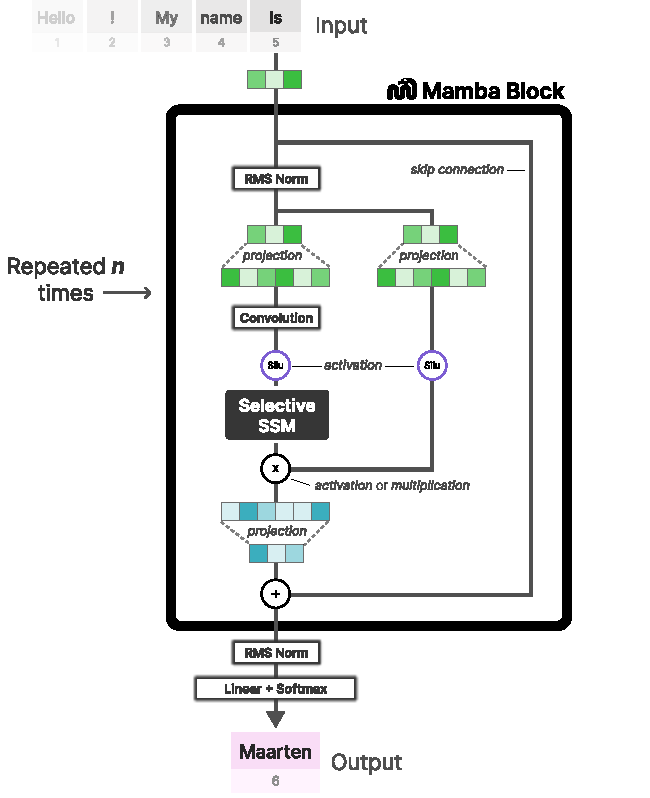
\includegraphics[width=\textwidth]{figures/3_theoretical_background/deep learning/mamba.pdf}
            \end{figure}
        \end{column}
    \end{columns}
\end{frame}